\chapter{Análise Bibliográfica sobre NLP, por Vitor de Oliveira Araujo Araruna\label{chap:bibliometria:vitorararuna}}

\section{Planejamento do estudo}

\textit{NLP} (natural language processing) ou processamento de linguagem natural (PLN em português) é a tecnologia usada para ajudar dispositivos tecnológicos a entenderem a linguagem do ser humano de maneira a responder suas demandas.

Esse processo pode parecer simples para você que está acostumado a mexer no seu smartphone e nos aplicativos que o compõem, bem como realizar uma pesquisa no Google e receber uma resposta de qualidade, mas a verdade é que você e a tecnologia usam linguagens diferentes e é preciso um “tradutor automático” para permitir que vocês se entendam.

 Natural Language Processing (NLP) é uma vertente da Inteligência Artificial que estuda a capacidade e as limitações de uma máquina em entender a linguagem dos seres humanos. Ou seja, é uma interface entre a linguagem homem-máquina. Dessa forma, o objetivo do PLN é fornecer aos computadores a capacidade de entender e compor textos.
 
 Para que isso aconteça, passamos por diversas etapas de um pré-processamento, ou seja, ao recolher um texto ou uma base de textos nos quais queremos que a máquina entenda, vamos "limpar" ele de uma forma na qual eu compute somente as informações importantes.
 
Algumas das técnincas usadas para pré-processar um texto:
\begin{itemize}
    \item Tokenization -> Tokens são componentes textuais independentes e contemporâneos que têm alguma sintaxe definidae semântica. (frases, setenças, paragrafos) 
    \item Stop Words -> São palavras/letras no texto que são insignificantes para a compreensão do contexto e que também são palavras no qual os motores de busca ignoram em seus resultados, como por exemplo: a, agora, ainda, alguém, algum,, deles, depois, dessa, dessas, desse, etc.
    \item Stemming -> Aqui vamos analisar cada palavra individualmente e reduzi-la à sua raiz ou, como é chamado na técnica, ao seu stem. Uma característica dessa técnica é que ela pode reduzir a palavra a uma outra gramaticalmente incorreta, porém ainda com valor para nossa análise
\end{itemize}

\subsection{Uso do Bibliometrix e Biblioshiny}
Serão usadas a ferramenta e o \textit{workflow} proposto pelos autores do pacote Bibliometrix, conforme indica a figura ~\ref{fig:bibliometrix:workflow}.

\subsection{Limitações} O exercício relatado foi feito em 5 horas, utilizando a base de dados Web of Science (WoS)


\section{Coleta de dados\label{MASSA:coleta}}

A coleta de dados feita usando a base Web of Science (WoS) no dia 10 de janeiro de 2022, acessado por meio do Portal de Periódicos da CAPES.

As buscas formam feitas nas coleções \textbf{Science  Citation  Index  Expanded (SCI -EXPANDED)} e \textbf{Social  Sciences  Citation  Index (SSCI)}, que contém registros relativos a vários campos do conhecimento, no qual o SCI-EXPANDED foca mais na área das ciências exatas e naturais, enquanto que o SSCI indexa artigos da área das ciências sociais. Observe que os artigos nessas duas coleções são indexados desde 1945. 


\subsection{Explicação para os termos de busca usados\label{}}

A busca utilizou cláusulas que retornassem registros relacionados a \textit{PROCESSAMENTO DE LINGUAGEM NATURAL} (NLP) nos formatos visuais e auditivos.

\section{Análise dos dados}

\subsection{Filtragem de registros}

Para a filtragem, removemos registros indesejados, como por exemplo ivros, reviews de livros, entre outros. O objetivo era obter apenas os artigos completos, visto que a análise desse assunto é mais confiável por parte de artigos.

\subsection{Análise descritiva do \textit{dataset} }

A seguir, é feita uma análise bibliométrica descritiva do \textit{dataset} utilizando a função \texttt{biblioAnalysis} do Bibliometrix, que realiza diversos cálculos para levantar as taxas apresentadas. Mais informações mem 

As informações mais gerais sobre o \textit{dataset} são as seguintes:
\begin{description}
    \item [\textit{Timespan}] Os artigos filtrados foram publicados entre 1982 e 2022.
    \item [\textit{Sources (Journals, Books, etc)}] São 1371 fontes de informação que publicaram os artigos recuperados no \textit{dataset}.
    \item [\textit{Average years from publication}] A média do tempo de publicação dos artigos no \textit{dataset} é de 6,93 anos.
    \item [\textit{Average citations per documents}] Cada artigo no \textit{dataset} foi citado, em média 6.815 vezes.
    \item [\textit{Average citations per year per doc}] Após publicado, cada um dos artigos foi citado, em média, 0.8895 vezes por ano.
    \item [\textit{References}] O \textit{dataset} contém 42408 referências citadas.
    \item [\textit{Keywords Plus (ID)}] 1544 distintas palavras-chave do tipo Keywords Plus (ID) foram encontradas no \textit{dataset}.
    \item [\textit{Author's Keywords (DE)}] 4321 distintas palavras-chave indicadas pelos autores foram encontradas no \textit{dataset} .
    \item [\textit{Authors}] 6088 distintos nomes de autores foram encontrados no \textit{dataset} .
    \item [\textit{Author Appearances}] Os 7185 distintos (nomes de) autores foram encontrados 2.297 vezes, como autores de artigos.
    \item [\textit{Authors of single-authored documents}] Dentre os 7185 distintos (nomes de) autores encontrados, 182 deles editaram artigos individualmente, isso é, sem co-autores.
    \item [\textit{Authors of multi-authored documents}] Dentre os 7185 distintos (nomes de) autores encontrados, 5906 deles editaram artigos com um ou mais co-autores"
    \item [\textit{Single-authored documents}] Dentre os 1973 documentos presentes no \textit{dataset}, 196 foram escritos por um único autor, e os restantes foram elaborados em co-autoria.
    \item [\textit{Documents per Author}] Dentre os 7185 distintos (nomes de) autores, cada um publicou em média 0.324 artigos.
\end{description}

\subsection{Evolução da Produção Científica}

\begin{figure}
    \centering
    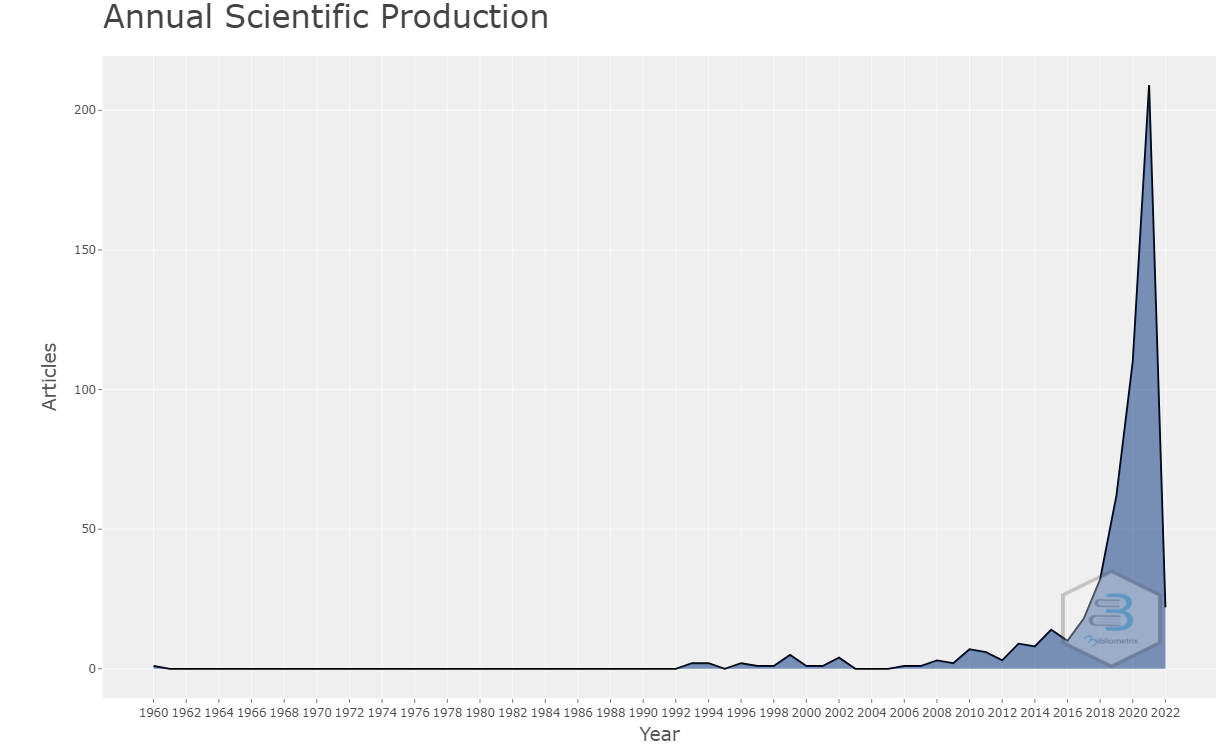
\includegraphics[width=1\textwidth]{experiments/titofrota/PesquisaBibliometrica/Deepfakes/annual-plot.png}
    \caption{Evolução da produção científica no \textit{dataset}}
    \label{fig:evol:anual:DEEPFAKES@titofrota}
\end{figure}

A figura \ref{fig:evol:anual:DEEPFAKES@titofrota} representa a evolução em produção científica mundial a respeito do tema NLP, de acordo com o \textit{dataset}. Houve um crescimento a notável a partir do ano de 2014, atingindo o pico em 2020. 
É perceptível que no \textit{dataset} ainda há artigos não relacionados ao tema analisado.

\subsection{Interpretação do Crescimento} a taxa de crescimento do \textit{dataset} demonstra que o tema tem chamado muita atenção nos últimos anos, provavelmente devido aos avanços nos estudos de Inteligência Artificial, juntamente com o interesse em fazer a máquina compreender a comunicação humana. \textit{deepfakes}.

\subsection{Evolução das Citações}

\begin{figure}
    \centering
    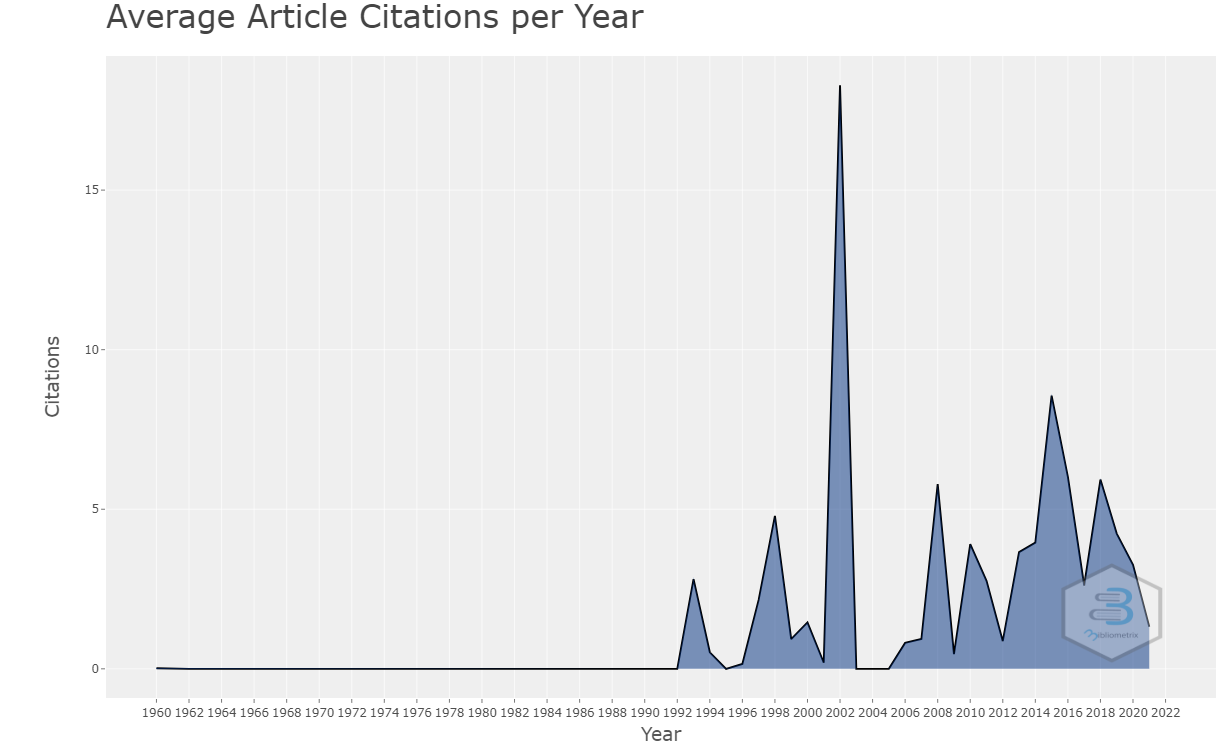
\includegraphics[angle=0,width=1\textwidth]{experiments/titofrota/PesquisaBibliometrica/Deepfakes/citations-year-plot.png}
    \caption{Evolução das citações ao \textit{dataset}.}
    \label{fig:evol:anual:citacoes:DEEPFAKES@titofrota}
\end{figure}

A figura \ref{fig:evol:anual:citacoes:DEEPFAKES@titofrota} apresenta a evolução da média de citações aos artigos do \textit{dataset}. Não há muita estabilidade na média anual de citações, até mesmo nos anos mais recentes. Porém percebe-se um pico entre os anos de 2010 e 2012.

\subsection{Interpretação das Citações}
Embora seja perceptível o aumento de publicações anuais no decorrer dos anos, é notório que há uma disparidade em relação às citações, uma vez que essa seja instável. Portanto assim, idealizando o fato de que o tema ainda é novo e precisa ser desenvolvido por parte dos cientistas.

\subsection{\textit{Three-Field Plots (Sankey diagram)}}

As \textit{Three-Field Plots (Sankey diagram)} (plotagens do tipo ``Três Campos'') correlacionam três conjuntos de atributos em busca das afinidades encontradas no \textit{dataset}. Assim, são demonstrados os principais fluxos entre diferentes conjuntos. Tais conjuntos são: autores (centro), referência citadas (esquerda) e palavras-chave (direita) mais importantes.


\begin{figure}
    \centering
    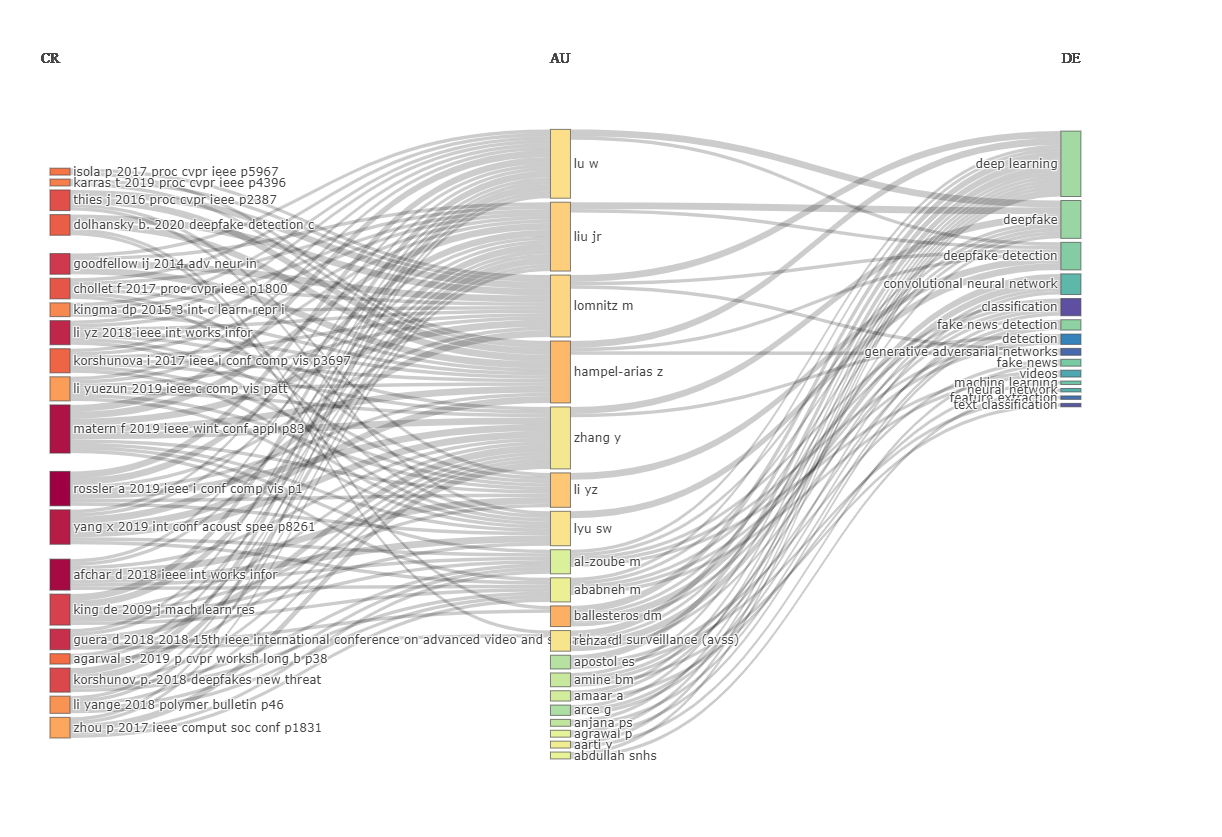
\includegraphics[width=1\textwidth]{experiments/titofrota/PesquisaBibliometrica/Deepfakes/ThreeFieldPlot.png}
    \caption{Plotagem do tipo``Três Campos'' (Sankey plot) do \textit{dataset}}
    \label{fig:DEEPFAKES@titofrota:ThreeFieldPlot}
\end{figure}

\subsection{Interpretação da figura \ref{fig:DEEPFAKES@titofrota:ThreeFieldPlot}}
A maioria dos autores mais relevantes apresentados na plotagem são, aparentemente, de origem oriental, mais especificamente chinesa. O que sugere o avanço e a preocupação do oriente a respeito do processamento de linguagem natural. Além disso, pode ser devido à dificuldade dos mesmos em se comunicar com outras linguas.


\section{Refinamento da Coleta de Dados}

Após a análise do \textit{dataset}, foi possível notar que praticamente a maioria dos artigos condizia para que a busca retornasse o esperado. Isso de faz por conta do termo de busca ter sido "NLP", setença que é intimamente ligada ao assunto de processamento de linguagens naturais e sem correspondência com outros assuntos. Devido à sua unicidade e originalidade do termo.

\section{Nova Análise dos Dados}

\subsection{Nova filtragem de registros}

Como os resultados condiziam com o esperado, decidi que para a nova filtragem seriam resgatados apenas os artigos considerados entre 2010 e 2012, onde houeram 2 picos de citações por parte dos cientistas, assim como os picos de criação de artigos por parte deles.


\subsection{Análise descritiva do \textit{dataset} refinado}

\begin{table}[]
    \centering
\csvautotabular[separator=semicolon
%,filter not strcmp={\csvcolii}{}
]{experiments/titofrota/PesquisaBibliometrica/Deepfakes/main-info.csv}
    \caption{Principais dados descritivos do dataset refinado.}
    \label{tab:DEEPFAKE:Main}
\end{table}

Logo, de acordo com a tabela \ref{tab:DEEPFAKE:Main}, é possível notar que entre 2017 e 2022 houveram 240 artigos publicados em 94 revistas diferentes.